\clearpage
\section{Quantum Oblivious Key Distribution with Discrete Variables}

\begin{tcolorbox}	
\begin{tabular}{p{2.75cm} p{0.2cm} p{10.5cm}} 	
\textbf{Student Name}  &:& Mariana Ramos\\
\textbf{Starting Date} &:& September 18, 2017\\
\textbf{Goal}          &:& Quantum oblivious key distribution (QOKD) implementation with discrete variables.\\
\textbf{Directory}     &:& sdf/ot\_with\_discrete\_variables.
\end{tabular}
\end{tcolorbox}

Oblivious Transfer (OT) is a fundamental primitive in multi-party computation. The one-out-of-two OT consists in a communication protocol between Alice and Bob. At the beginning of the protocol Alice has two messages $m_1$ and $m_2$ and Bob wants to know one of them, $m_b$, without Alice knowing which one, i.e. without Alice knowing $b$, and Alice wants to keep the other message private, i.e. without Bob knowing $m_{\bar{b}}$. therefore two conditions must be fulfilled:
\begin{enumerate}
	\item{The protocol must be concealing, i.e at the beginning of the protocol Bob does not know nothing about Alice's messages, while at the end of the protocol Bob will learn the message $m_{b}$ chosen by him.}
	\item{The protocol is oblivious, i.e Alice cannot learn anything about Bob's choice, bit $b$, and Bob cannot learning nothing about the other message $m_{\bar{b}}$.}
\end {enumerate}

In order to implement OT between two parties (Alice and Bob) they must be able to exchange continuously oblivious keys, i.e a QOKD system must exist between them.

\subsection{Quantum Oblivious Key Distribution System (QOKD)}

In this section we are going to describe the Quantum Oblivious Key Distribution system (QOKD).
The QOKD system enables two parties (Alice and Bob) to share a set of keys. These keys have the particularity of being half right and half wrong. Only Bob knows which are right and wrong keys.

Considering a discrete variables implementation, both Alice and Bob agree with the following correspondence, where $+$ corresponds to \textit{Rectilinear Basis} and $\times$ corresponds to \textit{Diagonal Basis},

\begin{table}[H]
\centering
\begin{tabular}{c|c}
\textbf{\textit{Basis}}         &  \\ \hline
 0 & $+$ \\
 1 & $\times$ \\
\end{tabular}
\end{table}
Alice and Bob also agree with the bit correspondence for each direction for each basis. For \textit{Rectilinear basis}, "$+$",

\begin{table}[H]
\centering
\begin{tabular}{c|c}
            & Basis "+" \\ \hline
 0 & $\to (0^{\circ})$ \\
 1 & $\uparrow (90^{\circ})$ \\
\end{tabular}
\end{table}
and for \textit{Diagonal Basis}, "$\times$",

\begin{table}[H]
\centering
\begin{tabular}{c|c}
      & Basis "$\times$" \\ \hline
 0 & $\searrow (-45^{\circ})$ \\
 1 & $\nearrow (45^{\circ})$ \\
\end{tabular}
\end{table}

\begin{enumerate}
  \item The first step is to establish for both Alice and Bob the block length $l$. In this case, lets assume $l=16$. Alice randomly generate a bit sequence with length $l$.
      Therefore, she must define two sets randomly: $S_{A1}$ which contains the basis values; and $S_{A2}$, which contains the key values.

      In that case, lets assume she generates the following sets $S_{A1'}$ and $S_{A2'}$:
      $$S_{A1'} = \{0,0,1,1,1,0,0,1,1,0,0,1,1,1,0,1 \},$$
      $$S_{A2'} = \{1,1,1,0,0,0,0,0,1,1,0,0,1,0,1,1 \}.$$

  \item Next, Alice sends to Bob throughout a quantum channel $l$ photons encoded using the basis defined in $S_{A1'}$ and according to the key bits defined in $S_{A2'}$.

      Therefore, in the current example, Alice sends the following photons,

      \begin{align*}
        S_{AB} & = \{\space { }\uparrow \ \space { }\space { },\space { }\uparrow \ \space { }\space { }, \space { }\nearrow \ \space { }\space { },\space { } \searrow \ \space { }\space { } \ , \space { }\searrow \ \space { }\space { }, \to \ , \to \ ,\space { } \searrow \ \space { }\space { },\space { } \nearrow \ \space { },\space { }\uparrow \ \space { }\space { }, \space { }\to \ ,\space { } \searrow\space { }\space { },\space { }\nearrow\space { }\space { },\space { }\searrow \ \ \space { }\space { },\space { }\uparrow \ \space { }\space { },\space { }\nearrow \space { }\space { }\} \\
          & =\{90^{\circ},90^{\circ}, 45^{\circ}, -45^{\circ},-45^{\circ}, 0^{\circ}, 0^{\circ}, -45^{\circ}, 45^{\circ},90^{\circ}, 0^{\circ}, -45^{\circ}, 45^{\circ}, -45^{\circ}, 90^{\circ}, 45^{\circ} \}.
        \label{eq:photonsalice}
      \end{align*}


  \item Bob also randomly generates $l=16$ bits, which are going to define his measurement basis, $S_{B1'}$. Lets assume,
        \begin{align*}
             S_{B1'} & = \{0 \ ,1 \ ,1 \ ,0 \ ,0 \ ,1 \ ,0 \ ,1 \ ,1 \ ,0 \ ,1 \ ,1 \ ,0 \ ,0 \ ,0 \ ,1 \  \} \\
                    & = \{ +,\times,\times,+,+,\times,+,\times, \times,+, \times, \times \,+,+,+,\times \}.
        \end{align*}

      Bob will get $l$ results:
      $$S_{B2'} = \{1,-,\underline{0},0,-,1,\underline{1},-,1,-,1,0,1,1,\underline{0},1 \}.$$

      The "$-$"\space{ } corresponds to no clicks in Bob's detector, due to attenuation. The underlined values are bits which were measured with a correct basis but an error has occurred due to imperfections in the quantum communication system.

  \item Bob is going to send a "$-1$"\space{ } or a hash value to Alice for each measurement that he performed, thereby being "$-1$"\space{ } the measurements which correspond to no clicks. In this case, we are going to assume that the hash value is calculated using the \textit{SHA-256} algorithm \cite{Liu2009}. In detail, Bob has two sets $S_{B1'}$ and $S_{B2'}$ and he is going to generate the set $S_{BH1}$ with $l$ values ("$-1$"\space{ } or hash values calculated for each position of $S_{B1'}$ with the correspondent position of $S_{B2'}$). Therefore, Bob will send to Alice the following set:
      $$S_{BH1}=\{{S}_{1},-1,{S}_{2},{S}_{3}, -1,{S}_{4},{S}_{5},-1,{S}_{6},-1,{S}_{7},{S}_{8},{S}_{9},{S}_{10},{S}_{11},{S}_{12} \}.$$


  \item Since Alice has received the confirmation of measurement from Bob, i.e after Alice has received $S_{BH1}$, she sends throughout a classical channel the basis which she has used to codify the photons updated with the information about the no received photons, $$S_{A1'} = \{0,-1,1,1,-1,0,0,-1,1,-1,0,1,1,1,0,1 \}$$.

      Due to attenuation, the previous sets are reduced to the length $12$ and they shall be replaced by the following:
      $$S_{A1}=\{0,1,1,0,0,1,0,1,1,1,0,1 \},$$
      $$S_{A2}=\{1,1,0,0,0,1,0,0,1,0,1,1 \},$$
      $$S_{B1}=\{0,1,0,1,0,1,1,1,0,0,0,1 \},$$
      $$S_{B2}=\{1,\underline{0},0,1,\underline{1},1,1,0,1,1,\underline{0},1 \}$$
      Note that $S_{B2}$ still has errors.

  \item In order to know which photons were measured correctly, Bob does the operation $S_{B3}=S_{B1} \oplus S_{A1}$.
      In the current example,

  \begin{table}[H]
    \centering
    \begin{tabular}{c|c c c c c c c c c c c c }
     $S_{B1}$ & 0 & 1 & 0 & 1 & 0 & 1 & 1 & 1 & 0 & 0 & 0 & 1\\
     $S_{A1}$ & 0 & 1 & 1 & 0 & 0 & 1 & 0 & 1 & 1 & 1 & 0 & 1\\ \hline
     $\oplus$ & 1 & 1 & 0 & 0 & 1 & 1 & 0 & 1 & 0 & 0 & 1 & 1
    \end{tabular}
    \end{table}

      In this way, Bob gets $$S_{B3} = \{1,1,0,0,1,1,0,1,0,0,1,1 \}.$$ When Bob uses the right basis he gets the values correctly, apart from possible errors in transmission, when he uses the wrong basis he just guess the value. The values "1"\space{ } correspond to the values he measured correctly and "0" \space{ }to the values he just guessed.
      Thus, Bob is building two sets of keys, one with correct basis measurements values and other with the wrong basis measurement values that he just guessed.

      Thus, Bob has two pair of sets, one for the right basis,

      $$S_{B_{rp}}= \{1,2,5,6,8,11,12 \},$$ $$ S_{B_{rb}} = \{1,0,1,1,0,0,1 \},$$
      where $S_{B_{rp}}$ is the set of positions and $SB_{rb}$ is the set of bit values he measured for each position. The other pair is for photons he measured with the wrong basis and then he just guessed the values,
      $$S_{B_{wp}}= \{3,4,7,9,10 \},$$ $$S_{B_{wb}} = \{0,1,1,1,1 \},$$
      where $S_{B_{wp}}$ is the set of positions and $S_{B_{wb}}$ is the set of bit values he measured for each position.

      Nevertheless, due to errors in transmission, some bits in $S_{B_{rb}}$ may be not right.

      At this point, in order to test Bob's honesty and to estimate the \textit{QBER} of the channel, Alice is going to ask Bob to open some pairs of the Bob's sets. The definition of the protocol to test Bob's honesty is still an open issue. However, depending on the \textit{QBER} estimated by her, Alice must have a parameter to set the number of right position she wants to open, i.e she must open a minimum number of right position in order to guarantee a minimum \textit{QBER}. This will increase the security of the protocol. Alice chooses some positions to open and tells Bob which positions she wants to open. Bob sends to Alice the pairs she chose and then these pairs are eliminated from them sets. Lets assume she asked to open the positions $10$, $11$ and $12$. If she concludes Bob is not being honest, she stops the protocol and they must start it again. Otherwise, the protocol continues. Lets assume Alice has verified these pairs using the hash function committed by Bob and concluded that he is being honest. Therefore, she sends to Bob the \textit{QBER} estimated by her.

      Now, Bob has the previous sets replaced by the following,
      \begin{align*}
        S_{B_{rp}} & = \{1,2,5,6,8 \} \\
        S_{B_{rb}} & = \{1,0,1,1,0 \} \\
        S_{B_{wp}} & = \{3,4,7,9 \} \\
        S_{B_{wb}} & = \{0,1,1,1 \}
      \end{align*}


      Bob is going to use a modified version of \textit{Cascade algorithm} to correct the errors due transmission.

      \subsubsection{Modified version of Cascade Algorithm}
      The Cascade algorithm is often used with a key set where all values are supposed right. In this case, Bob has two pairs of sets, one with the position and bit values of photon he measured with the correct basis and other with position and bit values of photon he measured with the wrong basis. He only needs to apply the Cascade algorithm in the set that he measured the photons correctly \cite{Brassard1994}. However, he must apply a modified version of the Cascade in the other set in order to keep in secret from Alice which set corresponds to right and which set corresponds to wrong measurements.

      Bob randomly generates a bit value. If he gets $0$, he will send to Alice the set $\{ S_{B_{rp}}, S_{B_{wp}}\}$. Otherwise, if he gets $1$ he will send the set $\{S_{B_{wp}}, S_{B_{rp}}\}$. This guarantee that Alice does not know which is the right or wrong set. Lets assume this random bit is "0" and he sends $\{S_{B_{rp}}, S_{B_{wp}}\}$.

      \begin{enumerate}
        \item Bob starts by applying the normal cascade to the set $S_{B_{rb}}$. After both know the error estimative Bob determine if the error rate is above the fail threshold. If it is truth they must start the procedure again. Lets assume the estimated error rate is acceptable. Bob and Alice use a random permutation which is represented in figure \ref{cascadepermutation} for a larger number of bits (agreed at the beginning) by applying it to the shifted keys, in order to guarantee the spread out of the error bits randomly and to separate consecutive errors from each other.

            \begin{figure}[h]
            	\centering
            	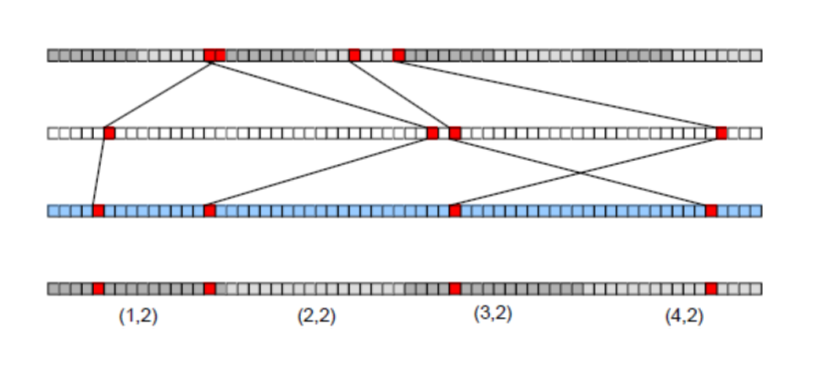
\includegraphics[width=0.6\textwidth, height=4cm]{./sdf/ot_with_discrete_variables/figures/cascade_permutation.png}
                	\caption{Cascade Algorithm - permutation}\label{cascadepermutation}
            \end{figure}

        \item Bob and Alice divide all the shifted key bits into blocks of N bits depending on the estimated error rate in order to have one or no error per block. In general, the sets of keys are too large and it is easier to explain the algorithm based on a larger number of bits. Therefore, figure \ref{cascade_1} represents the typical cascade initial steps. However, in this case, the set to be corrected only has five bits, therefore they divide the set in two sub-blocks, one with $3$ bits and other with $2$ bits.

             \begin{figure}[h]
            	\centering
            	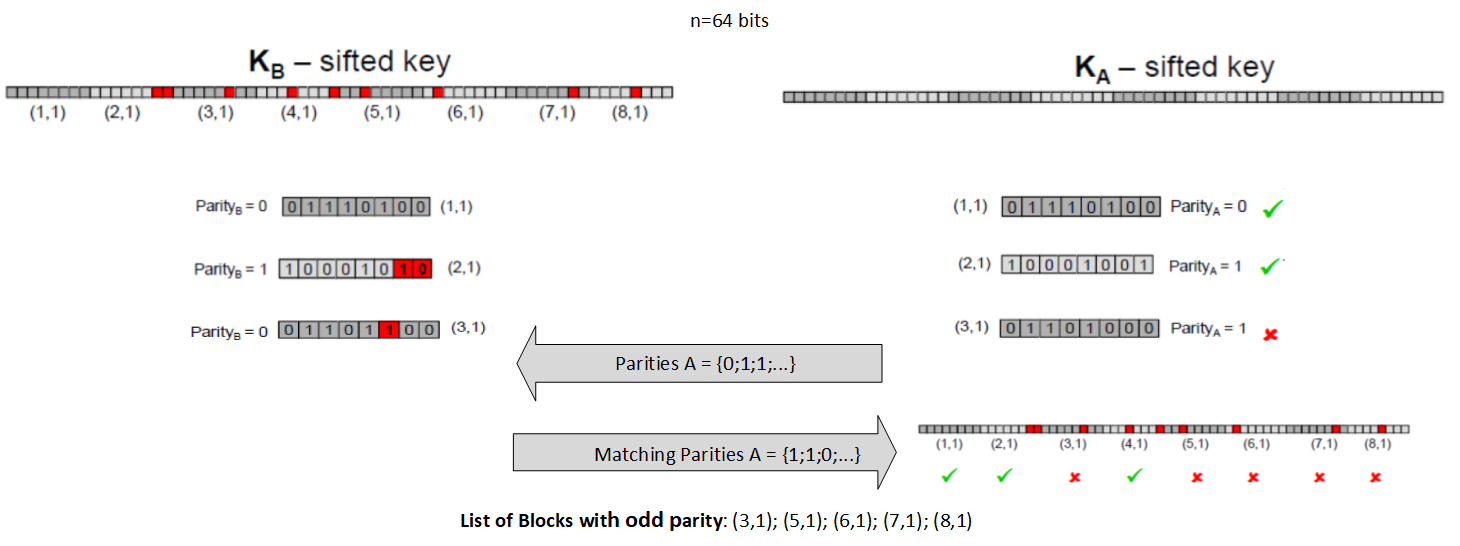
\includegraphics[width=0.8\textwidth, height=6cm]{./sdf/ot_with_discrete_variables/figures/cascade_1.png}
                	\caption{Cascade Algorithm}\label{cascade_1}
            \end{figure}

        \item They use a classical channel to compare the block parities. For blocks with different parities, an odd number of errors must exist, otherwise an even number of errors would mask each other. Thus, the block in which the parities disagree is divided in half into two smaller blocks of length $\frac{N}{2}$, and another parity check is performed on the first sub-block, as one can see in figure \ref{cascade_2}. As it was referred above, there is at least one error in one sub-block being the error location revealed by the parity of one sub-block. In other words, if the parity of the first sub-block passes, the error will be in the second sub-block. The sub-block with error will be sub-divided until the error is found.

            \begin{figure}[h]
            	\centering
            	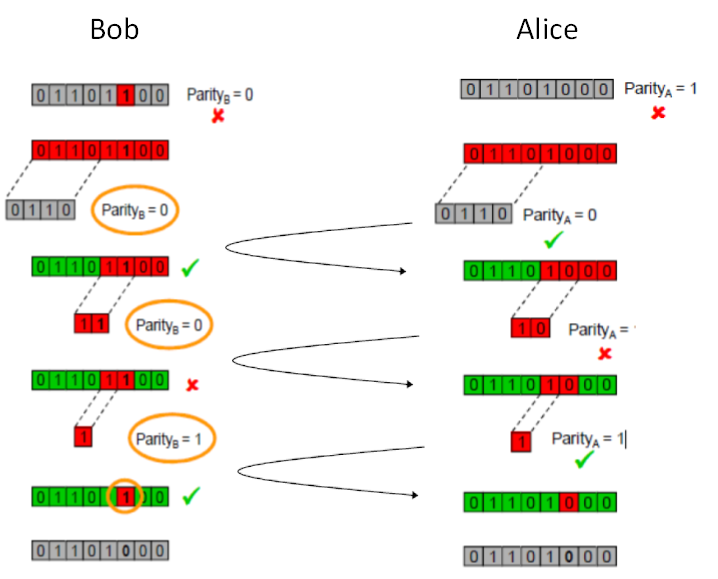
\includegraphics[width=0.6\textwidth, height=6cm]{./sdf/ot_with_discrete_variables/figures/cascade_2.png}
                	\caption{Cascade Algorithm - example of error correction}\label{cascade_2}
            \end{figure}

        \item When the error is corrected, the last bit of the block is discard in order to prevent the gain of additional information by Bob.


            In this case, lets assume the set of right positions was corrected with the algorithm described above and it will be replaced by the following:

            \begin{align*}
              S_{B_{rp}} & = \{1,2,5,6,8 \} \\
              S_{B_{rb}} & = \{1,1,0,1,0 \} \\
            \end{align*}

             In order to test Alice's honesty, Bob must verify if the \textit{QBER} sent by Alice is a realistic value. If it is not he stops the protocol and they must start again. Otherwise, the protocol continues.

      \end{enumerate}

      After that, Bob needs to apply the Fake Cascade to the set $S_{B_{wb}}$. The main goal of this step is to convince Alice she is performing the real Cascade but she is not.

      \begin{enumerate}
        \item First of all, based on the positions contained in $S_{B_{wb}}$, Bob must build an array with the correspondent bits in a random order and informs Alice the order of positions. In order to best explain this version of the algorithm, lets assume a larger set of bits.

            Bob sends to Alice throughout a classical channel the new positions order as if it were the permutation step represented in figure \ref{cascadepermutation} in real Cascade algorithm.

        \item Assuming each of them has a set with 32 bits randomly organized by Bob, they divide the supposed shifted keys in blocks with N bits according to the estimated error rate. As the \textit{QBER} is the same as for real cascade, Bob will assume the same number of errors, even if he starts for this modified version he can know the number of errors from \textit{QBER} estimated by Alice.

        \item Bob and Alice use a classical channel to compare the block parities. Alice sends to Bob her parity list. Based on Alice's parity list, Bob sends a block list with odd parities, i.e the blocks position in which parity supposed disagree. This list is randomly built based on the number of errors considered by Bob, i.e if he considered five errors from \textit{QBER} estimative, he will distributed them randomly and after that he will fill the remaining spaces with even parities. Bob sends to Alice the set with the list of odd parities, i.e the list of sub-sets he has different parities than Alice.

        \item The blocks with errors will be consecutively divided until they found the supposed errors. Since we have assumed there were five errors, this is the number of errors that Alice must supposedly correct.

            \begin{figure}[h]
            	\centering
            	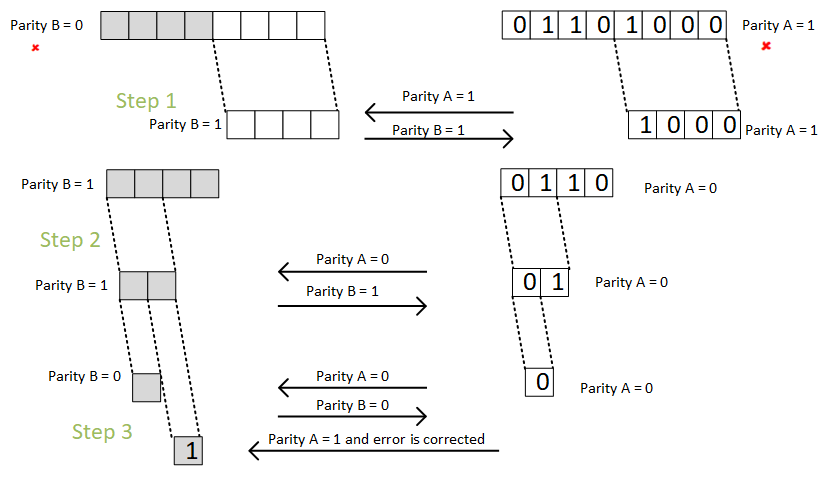
\includegraphics[width=0.6\textwidth, height=6cm]{./sdf/ot_with_discrete_variables/figures/fake_cascade.png}
                	\caption{Fake cascade - example of error correction}\label{fake cascade}
            \end{figure}

            Lets assume one of the blocks with error and analyse figure \ref{fake cascade}. Bob starts with a set filled with random bits, therefore we do not need to know which bits are. Alice starts by dividing her set in half with two blocks with $N$ bits.

            \begin{description}
              \item [Step 1:] Bob chooses one of the to blocks and informs Alice she must send the parity of this block. Lets assume he chose sub-block 2. She sends the parity and Bob is going to send his parity, which after know Alice's block parity he send the opposite parity. As referred in normal Cascade, there must be one error or no error in each block. Thus, since the parities disagree, the error must be in seconde block. They start the procedure to correct it.
              \item [Step 2:] Bob divides again the sub-block in half with $\frac{N}{2}$ bits and asks Alice for the parity of the first sub-block. She sends her parity equals to 0 and Bob sends to her the opposite parity again.

              \item [Step 3:] They divide the sub-block in half again and Bob asks Alice for the parity of the first bit. Alice sends to him the parity equals to her. As the error is not in the first be, it must be in the second, therefore Bob is able to correct this bit with the information sent by Alice.
            \end{description}

            Note that Bob make his choice of which half analyse first using a random bit generator result. If he got "0" \  he starts with the first half of the sub-block, otherwise, if he got "1", he starts with the second half. In addition, they must discard the last bit of each block and sub-block in which fake Cascade were applied in order to guarantee that Bob does not gain additional information.

            In this case, after apply the fake Cascade to $S_{B_{wb}}$, lets assume,
            \begin{align*}
                S_{B_{wp}} & = \{3,4,7,9 \} \\
                S_{B_{wb}} & = \{0,1,1,0 \}
            \end{align*}


      \end{enumerate}

      If Bob starts by applying the fake Cascade, he must test Alice's honesty at the beginning of the real Cascade application, based on the number of errors he has. If he thinks that the \textit{QBER} sent by Alice is unrealistic, he stops the protocol at this point.


  \item When Alice sends to Bob a photons set, they are building a set of pairs (array positions and bit values which correspond to measured photons at Bob's side and to the key bit with the photon was encoded at Alice's side).
      The main goal is to guarantee that Bob has the same number of right and wrong pairs. In addition, they must know information about $t$ (represented in figure \ref{alicebobkeys}) which corresponds to the points where the previous condition is verified.

      Since Bob has sent to Alice the information about the smallest set, in this example, Alice know that there are four pairs of wrong positions and five pairs of right positions. Alice must destroy one of the right pairs by asking Bob to open it. Therefore, at $t=8$ both know that there are the same number of right and wrong pairs thereby being the main goal guaranteed.

    \begin{figure}[h]
    	\centering
    	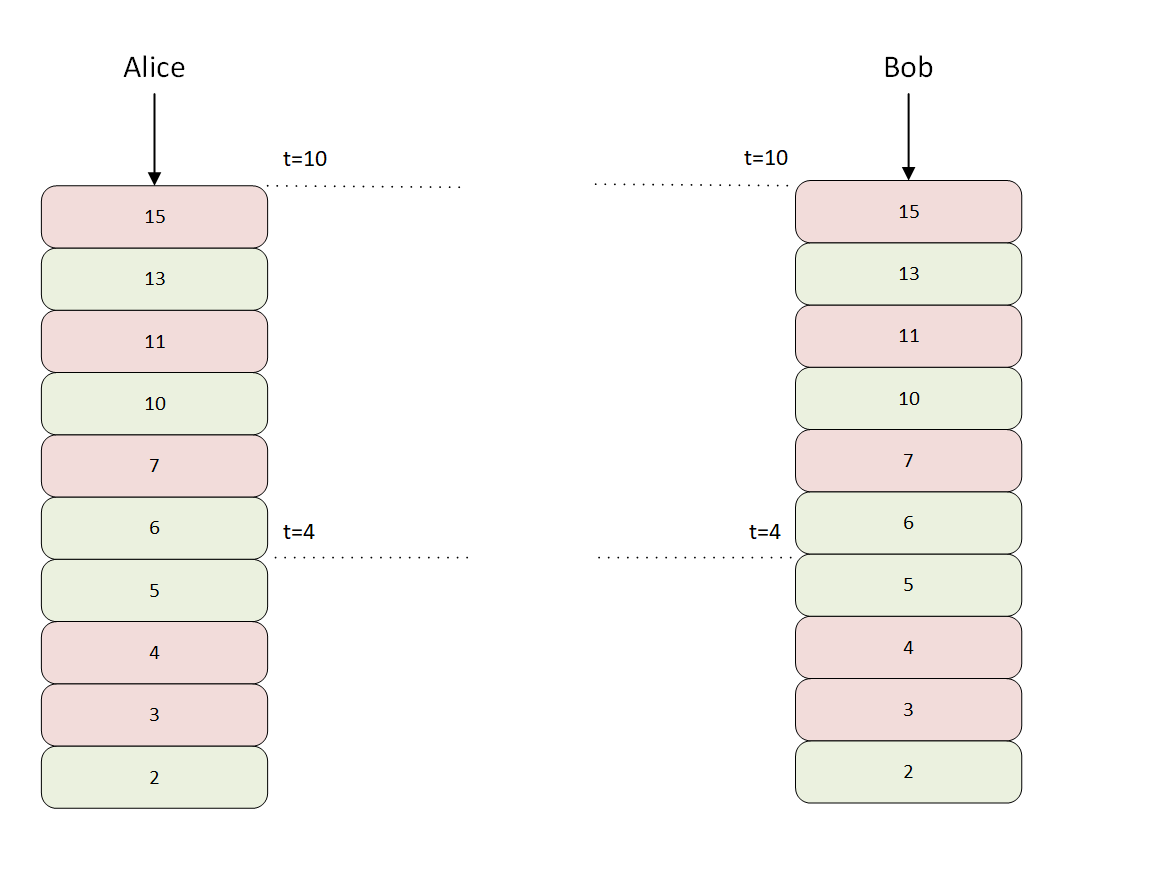
\includegraphics[width=1.0\textwidth, height=9cm]{./sdf/ot_with_discrete_variables/figures/alicebobkeys.png}
        	\caption{Alice and Bob key sets.}\label{alicebobkeys}
    \end{figure}

     As we can see in figure \ref{alicebobkeys}, unlike Bob, Alice does not know which positions corresponds to right or wrong measurements performed by Bob.
     They have been building these sets during all protocol.
\end{enumerate}

\subsection{OT Protocol with QOKD system}
    At this time, we are going to describe the oblivious transfer protocol with detail. As it was referred at the beginning, Alice sends two messages to Bob and he wants to know one of them. Alice does not know which message Bob wants and Bob only know the message he wants, i.e he does not know anything about the other message.
    Furthermore, only Alice knows information about messages $m_{0}$ and $m_{1}$.
    In this case, lets assume the following two messages with size $s=4$, $m_{0} = \{0 0 1 1\}$ and $m_{1} = \{0 0 0 1\}$.
    Alice must guarantee $t = s \times 2$. In order to do that, she must destroy the remaining pairs. In this case, there is no need to do that because they have a set for $t=8$ with the same number of wrong and right pairs.

  \begin{enumerate}
  \item Bob defines two new sub-sets, $I_{0}$ and $I_{1}$. $I_{0}$ is a set of values with photons array positions which Bob just guessed the measurement since he did not measure them with the same basis as Alice, $I_{1}$ is a set of values with photons array positions which Bob measured correctly since he used the same basis as Alice used to encoded them. The position of the pairs of each right and wrong message are in the keys sets that they have been building during the protocol.

  In this example, the message size is 4. Since, at this time $t=10$ and we have $5$ right pairs and $5$ wrong pairs, Alice ask to Bob to open one right pair and one wrong pair in order to both have exactly the message's size number of right and wrong pairs. Lets assume that Alice opened two pairs, position $15$ which is a wrong measurement and position $10$ which is a right measurement. We have now $t=8$.

  Next, Bob defines two sub-sets with size $s=4$:
  $$I_{0}=\{3,4,7,9 \},$$
  and $$I_{1}= \{1,2,6,8 \},$$ where $I_{0}$ is the sequence of positions in which Bob was wrong about basis measurement and $I_{1}$ is the sequence of positions in which Bob was right about basis measurement. Bob sends to Alice the set $S_{b}$

  Thus, if Bob wants to know $m_{0}$ he must send to Alice throughout a classical channel the set $S_{0}=\{I_{1},I_{0} \}$, otherwise if he wants to know $m_{1}$ he must send to Alice throughout a classical channel the set $S_{1}=\{I_{0},I_{1} \}$.


  \item Alice is sure about Bob's honesty, since she knows he only has $4$ right basis to measure the photons. In addition, Alice cannot know which message Bob chose because she did not know the order that he sent the sets.

  \item Lets assume Bob sent $S_{0}=\{I_{1},I_{0} \}$.
   Alice defines two encryption keys $K_{0}$ and $K_{1}$ using the values in positions defined by Bob in the set sent by him. In this example, lets assume: $$K_{0}=\{1,1,1,0\}$$ $$K_{1}=\{0,0,0,1\}.$$

   Alice does the following operations:
   $$m = \{m_{0}\oplus K_{0}, m_{1} \oplus K_{1} \}.$$

   \begin{table}[H]
    \centering
    \begin{tabular}{c|c c c c c c c c}
     $m_{0}$ & 0 & 0 & 1 & 1 \\
     $K_{0}$ & 1 & 1 & 1 & 0 \\ \hline
     $\oplus$ & 1 & 1 & 0 & 1
    \end{tabular}
    \end{table}

   \begin{table}[H]
    \centering
    \begin{tabular}{c|c c c c c c c c}
     $m_{1}$ & 0 & 0 & 0 & 1 \\
     $K_{1}$ & 0 & 0 & 0 & 1 \\ \hline
     $\oplus$ & 0 & 0 & 0 & 0
    \end{tabular}
    \end{table}

    Adding the two results, $m$ will be: $$m=\{1,1,0,1,0,0,0,0\}.$$

   After that, Alice sends to Bob the encrypted message $m$ through a classical channel.

  \item When Bob receives the message $m$, in the same way as Alice, Bob uses $S_{B1\prime}$ values of positions given by $I_{1}$ and $I_{0}$ and does the decrypted operation. In this case, he does following operation:

      \begin{table}[H]
        \centering
        \begin{tabular}{c|c c c c c c c c}
         $m$ & 1 & 1 & 0 & 1 & 0 & 0 & 0 & 0 \\
             & 1 & 1 & 1 & 0 & 0 & 1 & 1 & 0 \\ \hline
         $\oplus$ & 0 & 0 & 1 & 1 & 0 & 1 & 1 & 0 \\
        \end{tabular}
        \end{table}

      The first four bits corresponds to message 1 and he received $\{0,0,1,1\}$, which is the right message $m_{0}$ and $\{0,1,1,0\}$ which is a wrong message for $m_{1}$.


\end{enumerate}

\subsection{Simulation}

First of all, the protocol will be simulated and then a experimental setup will be built in the laboratory.

The main goal of this simulation is to demonstrate that Bob was able to learn correctly message $m_{b}$ and he does not know the message $m_{\overline{b}}$.

\begin{figure}[H]
	\centering
	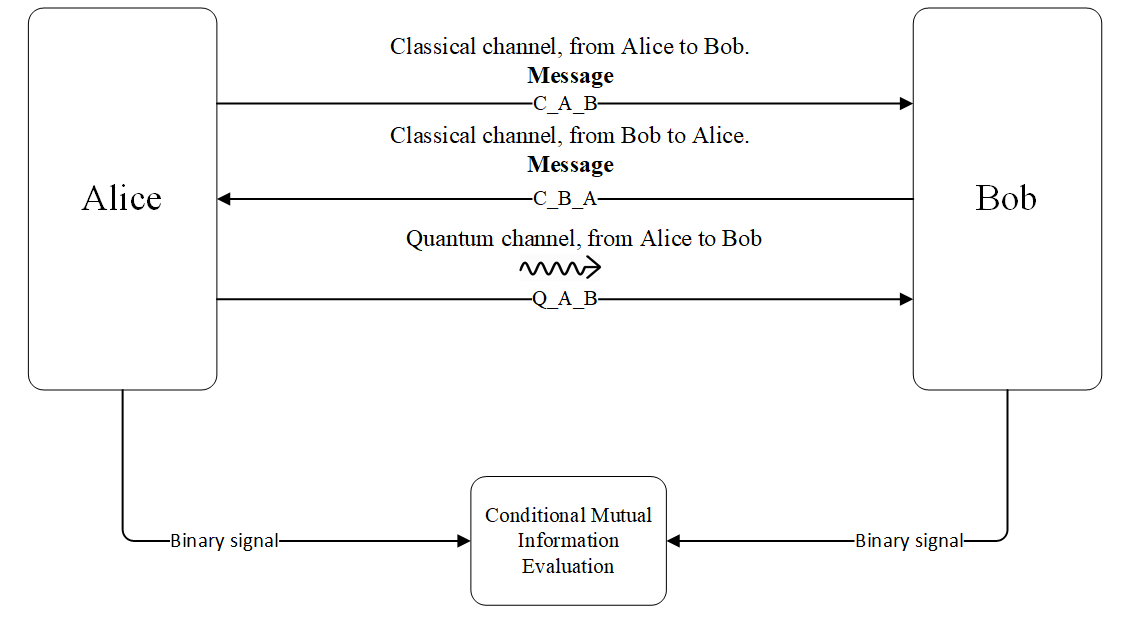
\includegraphics[width=1.0\textwidth, height=9cm]{./sdf/ot_with_discrete_variables/figures/Simulation_diagram_top.png}
	\caption{Simulation diagram at a top level}\label{toplevelsimulation}
\end{figure}

As one may see in figure \ref{toplevelsimulation} this simulation will have three top level blocks. Two of them are Alice and Bob and they are connected through two classical channels and one quantum channel. In addition, a third block will be performed in order to calculate the \textit{Mutual Information}. The mutual information (MI) between Alice and Bob is defined in terms of their join distribution.


\begin{enumerate}
  \item

  \begin{figure}[h]
	\centering
	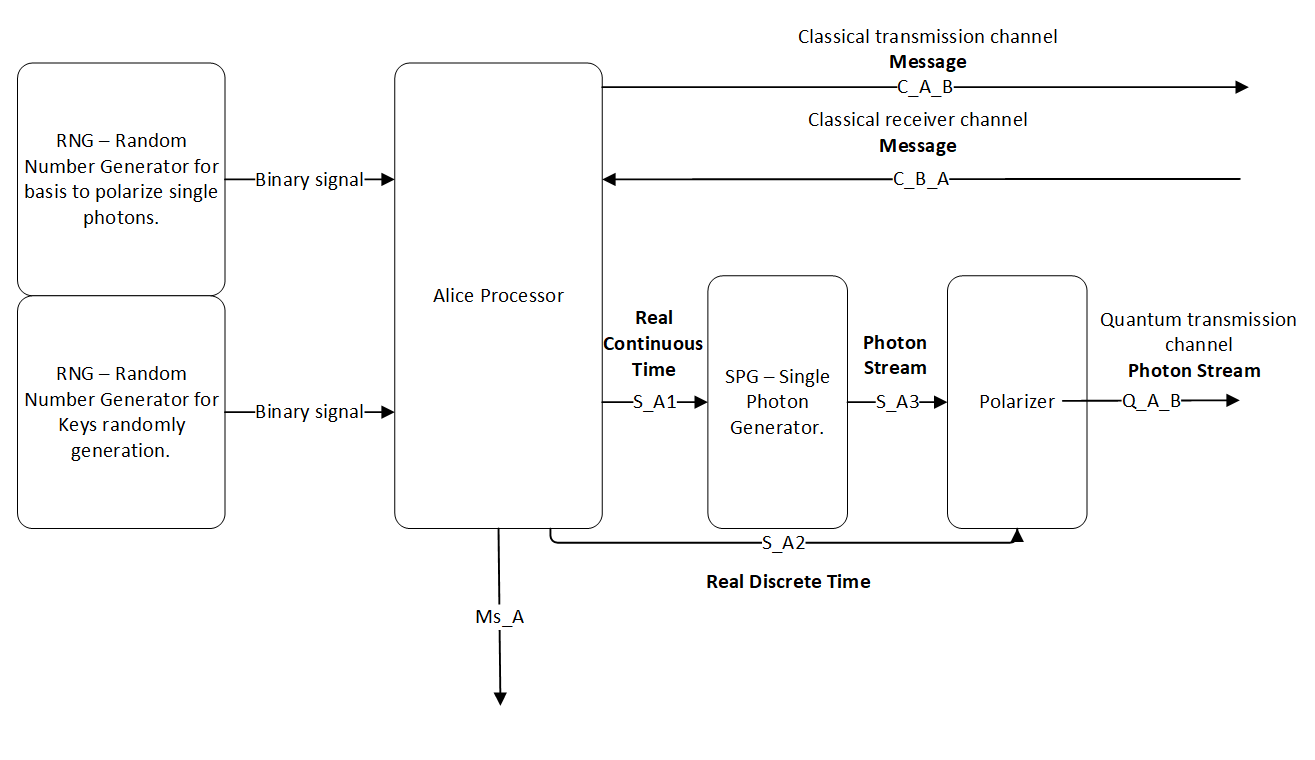
\includegraphics[width=1.1\textwidth, height=9cm]{./sdf/ot_with_discrete_variables/figures/Simulation_Alice.png}
	\caption{Simulation diagram - Alice's side}\label{simulationalice}
\end{figure}

    In figure \ref{simulationalice} one can observe a block diagram of the simulation at Alice's side. As it is shown in the figure, Alice must have one block for random number generation which is responsible for basis generation to polarize the photons, and for key random generation in order to have a random state to encode each photon. Furthermore, she has a Processor block for all logical operations: array analysis, hash function results validation, random number generation requests, and others. This block also receives the start information, i.e. message size s and messages $m_{0}$ and $m_{1}$, as well as information from Bob, i.e sets $I_{0}$ and $I_{1}$, hash function results, and others. In addition it is responsible for set the initial length $l$ of the first array of photons which will send to Bob. This block also must be responsible for send classical information to Bob. Finally, Processor block will also send a real continuous time signal to single photon generator, in order to generate photons according to this signal, and finally this block also sends to polarizer a real discrete signal in order to inform the polarizer which basis it should use. Therefore, she has two more blocks for quantum tasks: the single photon generator and the polarizer block which is responsible to encode the photons generated from the previous block and send them throughout a quantum channel from Alice to Bob.

    Finally, Alice's processor has an output to Mutual Information top level block, $Ms_{A}$.


  \item

  \begin{figure}[h]
	\centering
	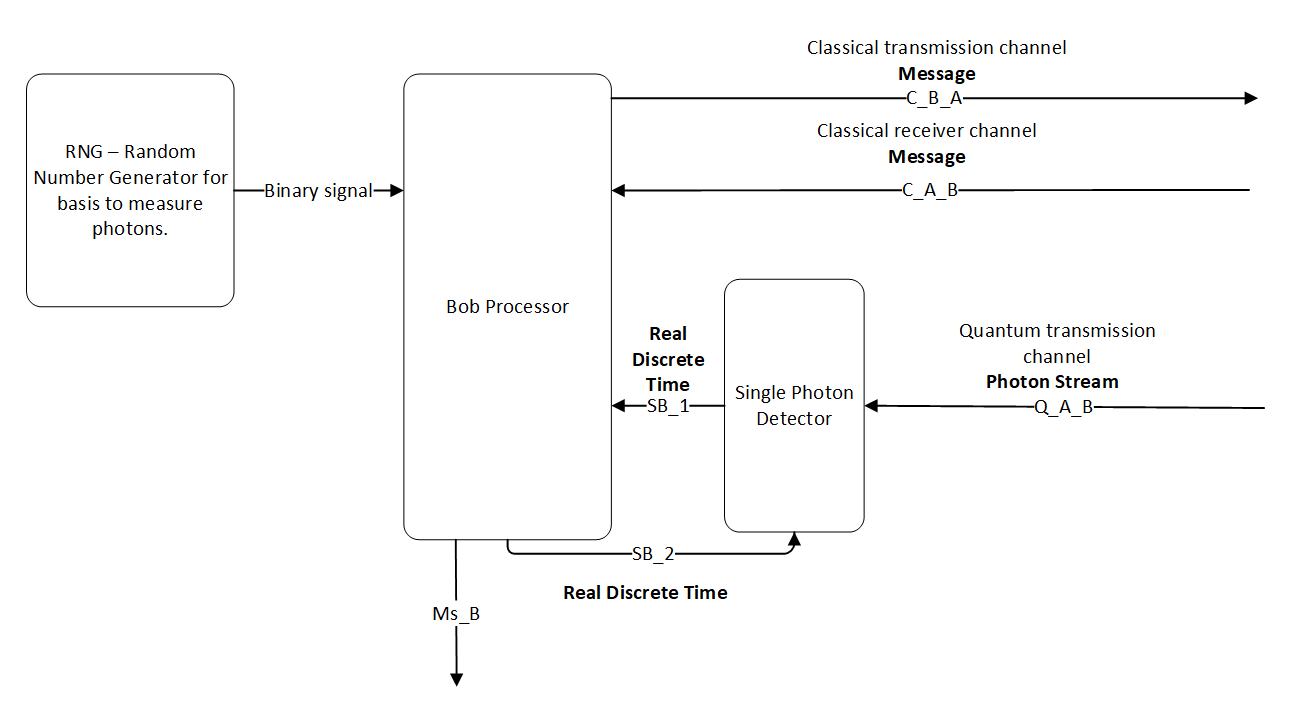
\includegraphics[width=1.1\textwidth, height=9cm]{./sdf/ot_with_discrete_variables/figures/Simulation_Bob.png}
	\caption{Simulation diagram - Bob's side}\label{simulationbob}
\end{figure}

    In figure \ref{simulationbob} one can observe a block diagram of the simulation at Bob's side. From this side, Bob has one block for Random Number Generation which is responsible for randomly generate basis values which Bob will use to measure the photons sent by Alice throughout the quantum channel. Furthermore, this Block will generate the random bits that Bob needs in Modified Version of Cascade Algorithm. Like Alice, Bob has a Processor block responsible for all logical tasks, i.e Hash function generation, analysing functions, requests for random number generator block, etc. Additionally, it receives information from Alice throughout a classical channel and a quantum channel but it sends information to Alice only throughout a classical channel. Furthermore, Bob has one more block for single photon detection which receives from processor block a real discrete time signal, in order to obtain the basis it should use to measure the photons.

    Finally, Bob's processor has an output to Mutual Information top level block, $Ms_{B}$.

  \item Mutual Information calculation

\end{enumerate}


\begin{table}[hbt]
\centering
\caption{System Signals}
\label{my-label}
\begin{tabular}{|l|l|l|}
\hline
\textbf{Signal name} & \textbf{Signal type} & \textbf{Status} \\ \hline
NUM\_A                &  Binary signal       &                 \\ \hline
NUM\_B                &  Binary signal       &                 \\ \hline
CLK\_A                &  Real continuous Time&                 \\ \hline
CLK\_B                &  Real continuous Time&                 \\ \hline
C\_A\_B                &  Message             &                 \\ \hline
C\_B\_A                &  Message             &                 \\ \hline
S\_A1                 &  Real continuous Time&                 \\ \hline
S\_A2                 &  Real discrete   Time&                 \\ \hline
S\_A3                 &  Photon Stream       &                 \\ \hline
Q\_A\_B                &  Photon Stream       &                 \\ \hline
Ms\_A                 &  Message             &                 \\ \hline
Ms\_B                 &  Message             &                 \\ \hline
S\_B1                 &  Real continuous Time&                 \\ \hline
S\_B2                 &  Real continuous Time&                 \\ \hline

\end{tabular}
\end{table}

\begin{table}[H]
\centering
\caption{System input parameters}
\label{my-label}
\begin{tabular}{|c|c|c|}
\hline
\textbf{Parameter} & \textbf{Default Value} & \textbf{Description}                   \\ \hline
messageSize                              & 4                                           & Size of the message Alice must send to Bob.\\ \hline
blockLenght                              & 16                                          & Block length.                                                  \\ \hline
systemRate                               &                                             &                                                 \\ \hline
\end{tabular}
\end{table}

\begin{table}[H]
\centering
\caption{Header Files}
\label{tab:headerfiles}
\begin{tabular}{|c|c|c|}
\hline
\textbf{File name}           & \textbf{Description}  & \textbf{Status}       \\ \hline
random\_number\_generator.h  &                       &                       \\ \hline
real\_continuous\_time.h     &                       &                       \\ \hline
real\_discrete\_time.h       &                       &                       \\ \hline
single\_photons\_generator.h &                       &                       \\ \hline
single\_photons\_detector.h  &                       &                       \\ \hline
encorder.h                   &                       &                       \\ \hline
decoder.h                    &                       &                       \\ \hline
message\_toSend.h              &                       &                       \\ \hline
message\_toReceive.h           &                       &                       \\ \hline
alice\_tasks.h               &                       &                       \\ \hline
Bob\_tasks.h                 &                       &                       \\ \hline
mutual\_information.h        &                       &                       \\ \hline
cascade\_truth.h               &                       &                       \\ \hline
cascade\_fake.h                &                       &                       \\ \hline
Sha256.h                     &                       &                       \\ \hline
\end{tabular}
\end{table}

\begin{table}[H]
\centering
\caption{Source Files}
\label{tab:sourcefiles}
\begin{tabular}{|c|c|c|}
\hline
\textbf{File name}           & \textbf{Description}  & \textbf{Status}       \\ \hline
random\_number\_generator.c  &                       &                       \\ \hline
real\_continuous\_time.c     &                       &                       \\ \hline
real\_discrete\_time.c       &                       &                       \\ \hline
single\_photons\_generator.c &                       &                       \\ \hline
single\_photons\_detector.c  &                       &                       \\ \hline
encorder.c                   &                       &                       \\ \hline
decoder.c                    &                       &                       \\ \hline
message\_toSend.c              &                       &                       \\ \hline
message\_toReceive.c           &                       &                       \\ \hline
alice\_tasks.c               &                       &                       \\ \hline
Bob\_tasks.c                 &                       &                       \\ \hline
mutual\_information.c        &                       &                       \\ \hline
QOKD\_main.c                 &                       &                       \\ \hline
cascade\_truth.c               &                       &                       \\ \hline
cascade\_fake.c                &                       &                       \\ \hline
Sha256.c                     &                       &                       \\ \hline
\end{tabular}
\end{table}

\subsection{Experimental}
In figures \ref{quantumchannelcommunication1} and \ref{quantumchannelcommunication2} are presented the experimental setup to be performed in the lab. Starting with Alice's side and then Bob's side. The main goal is to build an experimental setup in with Alice and Bob communicate through two classical channels and one quantum channel that will have only one direction (Alice to Bob).

\begin{enumerate}
  \item In figure \ref{quantumchannelcommunication1} is presented Alice's side in quantum communication. In order to generate single photons, we will start by using as light source a laser semiconductor with $1550nm$. After that, we need a \textbf{MPC} (manual polarization controller) to maximize the number of photons that output the \textbf{MZM} (Mach-Zehnder modulator). Next, there is an \textbf{OS} (Optical splitter 1 to 4, 25:25:25:25) which will split the light through the 4 arms equally.  Afterwards, there are four arms with a \textbf{MPC}, a \textbf{LP} (Linear Polarizer) which allows the photon passes through one of the considered basis, rectilinear ($0^{\circ}$ or $90^{\circ}$) or diagonal ($45^{\circ}$ or $-45^{\circ}$) and a \textbf{VOA} (Variable Optical Attenuator) in order to achieve the single-photon regime. Afterwards, there is a \textbf{Optical Demux 4x1}, which is connected to Alice Processor in order to receive a random number from the RNG contained in the processor, and according to the classical bit received the photon will go to the upper or down arm. This random number generated by Alice is '$0$' or '$1$' depending on the basis she wants use to encode the photon. After that, the photon follows its path to Bob through a quantum channel.


        \begin{figure}[H]
        	\centering 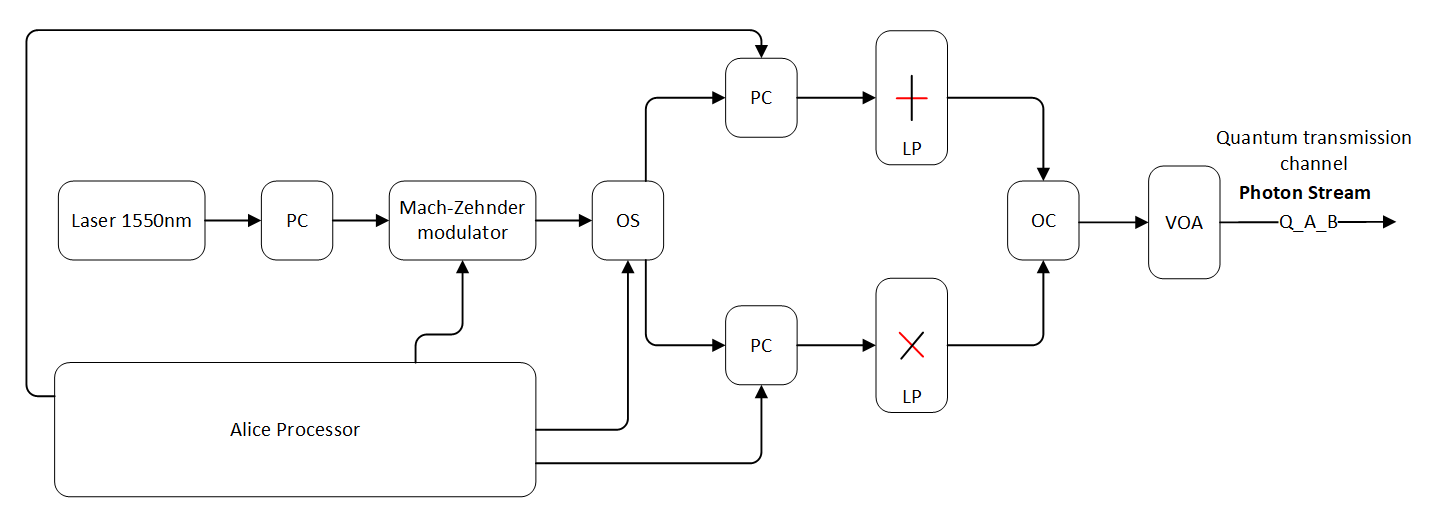
\includegraphics[width=1.1\textwidth,height=8cm]{./sdf/ot_with_discrete_variables/figures/experimental_alice.png}
        	\caption{Quantum communication diagram - Alice's side}\label{quantumchannelcommunication1}
        \end{figure}

  \item In figure \ref{quantumchannelcommunication2} is presented Bob's side in the quantum communication between he and Alice. The photons came to Bob's side through an optical fiber and it reaches an \textbf{OS} (Optical switch) controlled by Bob's processor which has a \textbf{RNG} (Random number generator) that chooses the basis Bob will use to measure the photons. This switch will forward the photon through the upper or lower arm. If photon goes through the upper arm, it will be measured using a linear basis. Otherwise, if it goes through the lower arm it will be measured using a diagonal basis. At the end, there are two detector \textbf{D1} and \textbf{D2} which are responsible to detect the photons that came and send a signal of measurement to Bob's processor.

        \begin{figure}[H]
        	\centering 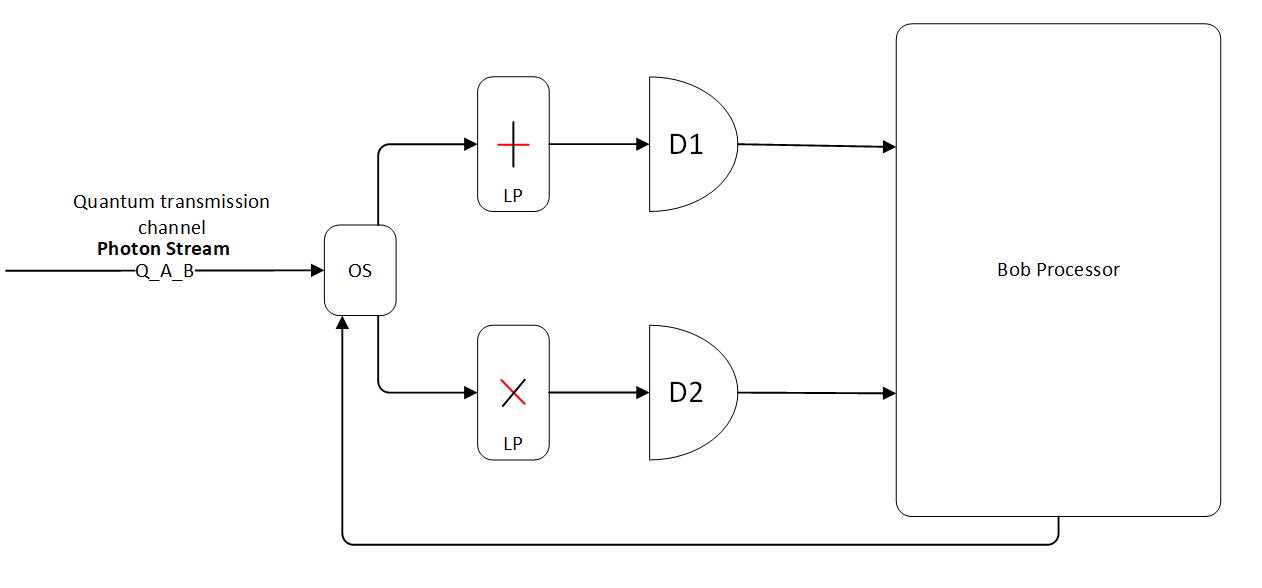
\includegraphics[width=1.0\textwidth,height=6cm]{./sdf/ot_with_discrete_variables/figures/experimental_bob.png}
        	\caption{Quantum communication diagram - Bob's side}\label{quantumchannelcommunication2}
        \end{figure}

\end{enumerate}

Furthermore, the two processors (Alice and Bob) must be able to communicate in a bi-directional classical channel to exchange all information that they need.

In table \ref{tb:mat} are described all components needed to build the experimental setup.

\begin{table}[hbt]
\centering
\caption{List of material}
\label{tb:mat}
\begin{tabular}{|c|c|c|}
\hline
\textbf{Material Name}     & \textbf{Quantity} & \textbf{Status} \\ \hline
Laser semiconductor 1550nm & 1                 &  \checkmark     \\ \hline
Manual polarization controller    & 5                 &       \\ \hline
       Linear Polarizer    & 6                 & \\ \hline
Mach-Zehnder Modulator     & 1                 &  \checkmark 2.56GHz   \\ \hline
Single Photon Detector     & 2                 &  \checkmark     \\ \hline
Optical Splitter           & 1                 &     \\ \hline
Optical switch            & 1                 &\checkmark, 5KHz-1MHz\\ \hline
Optical Demux 4x1 & 1                 &  \checkmark   50/50  \\ \hline
Variable Optical Attenuator & 4                 &  \checkmark     \\ \hline
Computer                    & 1                 &     \\ \hline
\end{tabular}
\end{table}


\bibliographystyle{unsrt}

\bibliography{bibliography}
